% !TEX root =  main.tex



\chapter{System Overview}
\label{chap:overview}
\pagestyle{plain}

This chapter presents the measures of similarity used in our system as well as giving a high-level introduction to the system's architecture, how it is set up in a distributed environment, how user can use it to query for similar datasets.

\section{Measures of similarity}\label{simMeasures}

As mentioned in section \ref{schemaMatching}, the task of similarity search is comparable to the task of schema matching, therefore, we also use schema matching techniques to measure the relatedness between two datasets. The system follows a hybrid schema matching approach, as both the schema and the instances are utilized.

\subsection{Schema similarity}\label{schemaSim}

First, the \textit{data type} of the attributes are used as a hard measurement for how similar the two attributes are, meaning if an attribute does not have a similar type to a query attribute, they are inherently dissimilar. Therefore, this attribute will be excluded from the candidate set, preventing further calculations with it.

Second, the \textit{table name} is considered in the similarity calculation. We provide two options on how a similar score between table names can be calculated:

\begin{itemize}
    \item \textbf{Q-gram sets similarity}: The syntactic similarity of two table names is calculated by measuring the Jaccard coefficient between their q-gram sets. By comparing their q-grams, the table names can be fuzzily matched, so that a table whose name is a typo of the query table's name can still be recognized as a candidate.
    \item \textbf{WordNet similarity}: Measures the similarity of the table names according to their semantics. The equation to the similarity calculation is mentioned in section \ref{wordnet}. This method requires however pair-wise calculations, since the semantic information of a word cannot be summarized into a sketch.
\end{itemize}

The last schema-level information taken into consideration is the \textit{attribute/column name}. The same methods of calculation for table name are also applied for this case.

\subsection{Instance similarity}

The two types of evidence inspected at the instance level are \textit{value sets overlap} and \textit{format overlap}. To calculate the similarity score, first we create a set from all the values of a column (i.e. retrieving a collection of unique values from the column).

For value sets overlap, the unique values sets are transformed into a MinHash sketch, on which the similarity calculation are performed. To avoid pair-wise comparison of all sketches, all sketches are added to a Lazo LSH index (section \ref{lazo}.

Format overlap, inspired by \cite{d3l}, relies on the format of the values to determine relatedness. The format of a value is a regular, predictable structure of the value string's representation, describable through a regular expression (regex). Using this approach, we are able to differentiate between a column of zip code (format: numbers) and a column of email (format: characters, followed by a special symbol "@" then characters, a dot and some more characters), for example. The details of how the regular expression are created are discussed in chapter \ref{chap:implementation}. From the unique values set, we create a set of all regular expressions that can describe all values of a column. The regex sets for all columns are also transformed into MinHash sketches, similar to the unique values sets above, and inserted into their own LSH index.

\section{System Architecture}\label{systemArchitecture}

The system consists of two main components: the client application and the server application. The client application should be run on machines where the query function is desired, while the server application is set up on one single machine, where it communicates with the database server and the clients can send their query requests to in order to be processed (figure \ref{fig:architecture}).

\begin{figure}[h]
    \centering
    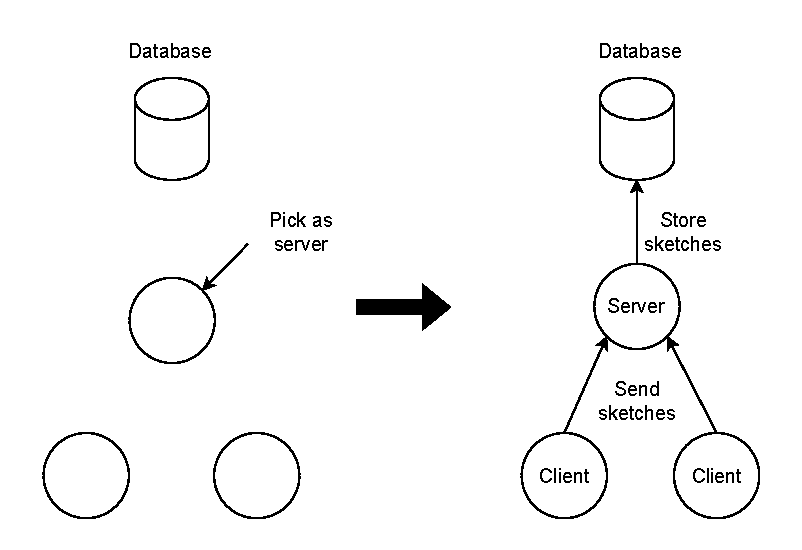
\includegraphics[scale=0.7]{architecture.pdf}
    \caption{Architecture overview}
    \label{fig:architecture}
\end{figure}

The rationale behind this set up is as follows: The goal of our system is to minimize the amount of data sent across the network, therefore the datasets should be locally processed to create a summary which is smaller in size and thus transferable over the internet. At this point, a server is not needed, since a machine can simply send the summaries to the database server to store and query the database to find similar datasets. However, as already discussed in section \ref{lsh}, pair-wise similarity calculations are costly, hence we use LSH for similarity search, specifically the Lazo implementation proposed by Bogatu et al. \cite{lazo}. Unfortunately, one drawback of Lazo is that the indexes are only capable of running in main memory, which we discuss in chapter \ref{chap:conclusion}. As a result, there needs to exist one central machine to store the LSH indexes. An alternative would be for all machines to store indexes, which would require all machines to retrieve new summary and update their indexes whenever new summaries enter the database, incurring unnecessary network traffic.

\section{Usage}

The system starts by letting an user from a machine boot up the server application, providing the application with the information of the host and port of the database server. Then, users from client machines boot up their respective client applications, providing the application on startup with the base IP address and port where the server can be reached. Were the server application to be moved to another machine, users from client-side boot up the application again with the new IP address and port. Once the server and client are both running, user can access a graphical interface from the web browser. From there, user can choose between two primary actions: upload and query.

\begin{itemize}
    \item \textbf{Upload action}: Submit datasets for the client application to process, create summaries and send to the server via REST request to store. In the interface, user can either choose to upload a single file, by providing the path from the file system to that exact file, or user can upload an entire folder of datasets by specifying the path to that folder (figure \ref{fig:upload}). Depending on the result of the action, the UI displays a success or error message.
    \item \textbf{Query action}: Submit a dataset for the client application to process, create summaries and send to the server via REST request to query. In the interface, user provide the path to the file to be queried, the limit on how many matches to receive, the threshold at which a candidate is considered a match and choose between the two query modes: join and union (figure \ref{fig:query}). If the action failed, an error will be displayed on the form interface, meanwhile a successful action will redirect the user to the result interface, where all matches are displayed in descending order of similarity score (\ref{fig:result}). 
\end{itemize}

\begin{figure}
    \centering
    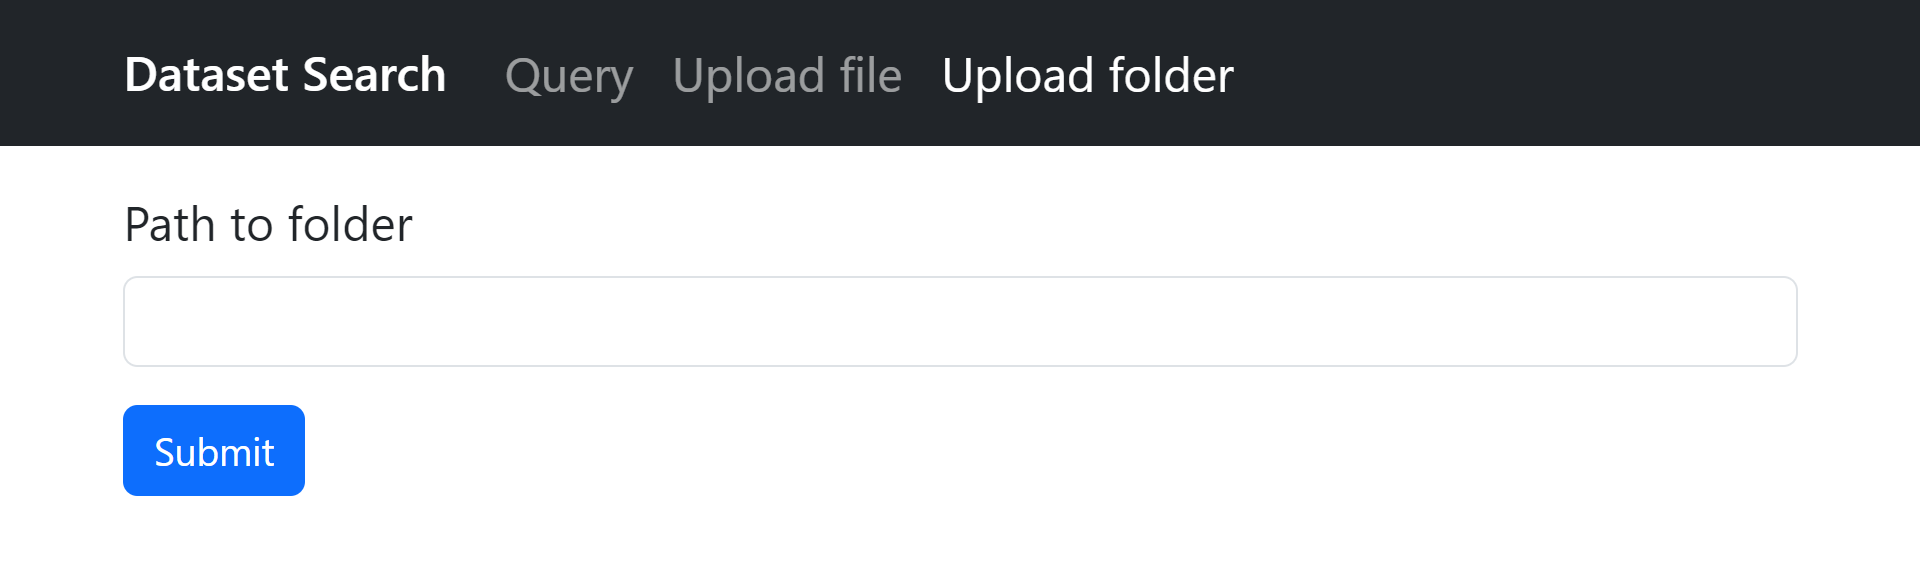
\includegraphics[width=\textwidth]{upload.png}
    \caption{Upload interface}
    \label{fig:upload}
\end{figure}

\begin{figure}
    \centering
    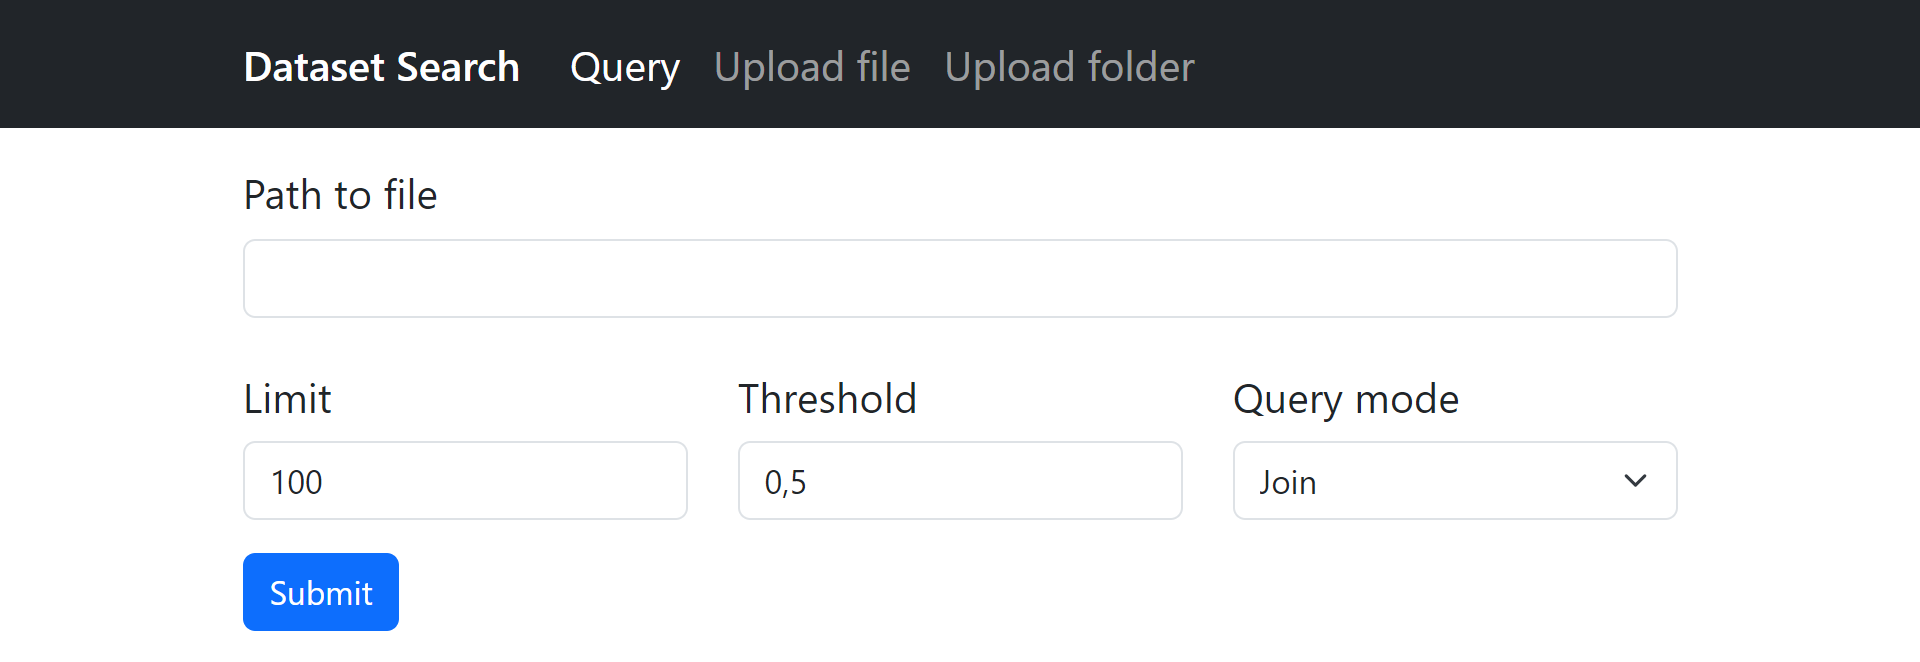
\includegraphics[width=\textwidth]{query.png}
    \caption{Query interface}
    \label{fig:query}
\end{figure}

\begin{figure}
    \centering
    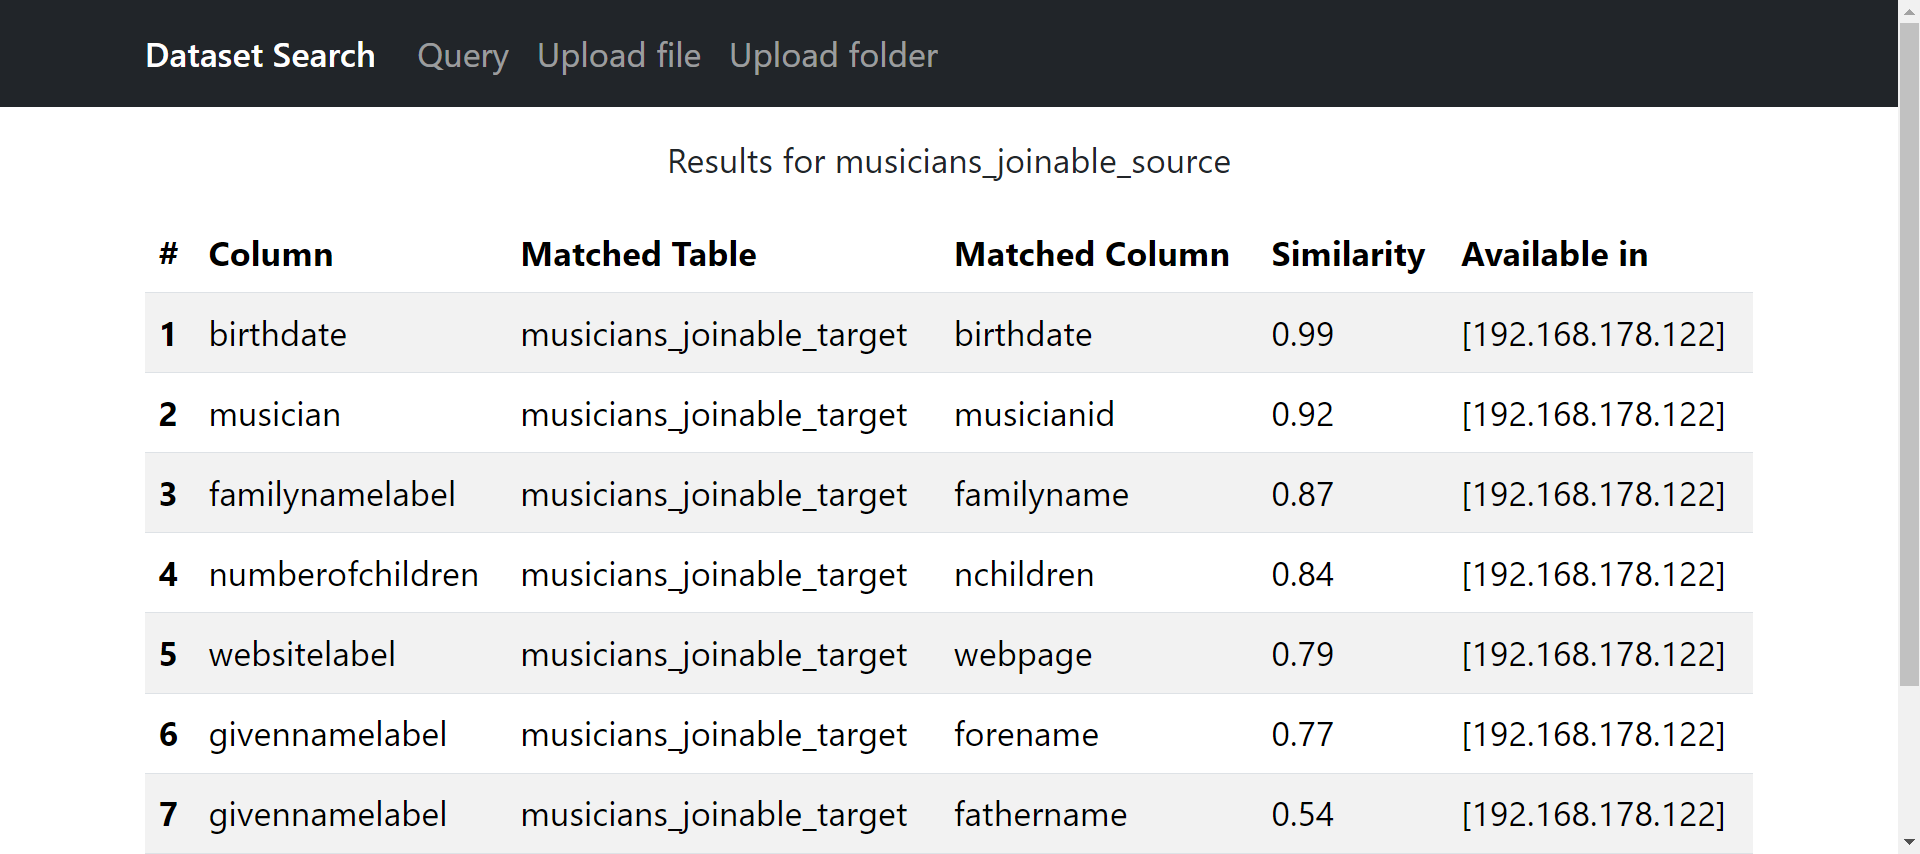
\includegraphics[width=\textwidth]{result.png}
    \caption{Result interface}
    \label{fig:result}
\end{figure}